\documentclass[a4paper,11pt]{report}
\usepackage[T1]{fontenc}
\usepackage[utf8]{inputenc}
\usepackage[italian]{babel}
\usepackage{graphicx}
\usepackage{amsfonts}
\usepackage{amsmath}
\usepackage{mathtools}
\usepackage{color}
\usepackage{geometry}
\geometry{a4paper, top=1.8cm, bottom=2cm, left=2cm, right=2cm}
\usepackage{hyperref}
\hypersetup{
	colorlinks=true,
	linkcolor=black,
	filecolor=blue,
	citecolor = black,      
	urlcolor=cyan,
}

\begin{document}
	\date{}
	\author{Marco Militello}
	\title{FISICA III}
	\maketitle
	\tableofcontents
	\newpage
	\section{Teoria cinetica}
		$\frac{m<v_x^2>}{2}=\frac{K_BT}{2} \Rightarrow <v_x^2>= \frac{K_BT}{m}$ \newline
		$<v_x^2> = \int_{-\infty}^{\infty} v_x^2 \frac{A}{\sqrt{\pi}}e^{-A^2v_x^2} = \frac{K_BT}{m} $ \newline
		$<v_x^2> = \frac{1}{2A^2} = \frac{K_BT}{m} \Rightarrow A=\sqrt{\frac{m}{2K_BT}}$ 
		
		\noindent $f(v_x^2)dv_x = \sqrt{\frac{m}{2\pi K_BT} e^{-\frac{mv_x^2}{2K_BT}dv_x}} \Rightarrow$ Gaussiana centrata in 0 con $\sigma^2 = \frac{K_BT}{M}$ [la velocità media è nulla] 
		
		\noindent Passando alle coordinate sferiche ($dxdydz = r\sin\theta d\phi r d\theta dr$) si ottiene la DISTRIBUZIONE DI MAXWELL-BOLTZMANN
		$$
		F(v)dv = 4\pi {(\frac{m}{2\pi K_BT})}^{\frac{3}{2}} v^2 e^{-\frac{m}{2K_BT}v^2} dv
		$$
		$n(v)dv = NF(v)dv$ numero di particelle con $v \in (v,v+dv)$
		\begin{figure}[h]
			\centering
			\includegraphics[width=0.7\linewidth]{immagini/Distibuzione velocità}
			\caption{Distribuzione asimmetrica delle velocità}
			\label{fig:distibuzione-velocita}
		\end{figure}
	
		\begin{itemize}
			\item Per ricavare $v_{mp}$ derivo la distribuzione rispetto a $v \Rightarrow v_{mp} = \sqrt{\frac{2K_BT}{m}}$
			\item $v_media= <v> = \sqrt{\frac{8K_BT}{\pi m}}$
			\item $v_{rms} = \sqrt{\frac{3K_BT}{m}}$
		\end{itemize}
		$v_{mp} < v_{media} < v_{rms}$
		\newpage
	\subsection{Esperimento selettore di velocità}
		\begin{figure}[h]
			\centering
			\includegraphics[width=0.7\linewidth]{immagini/"selettore velocità"}
			\caption{apparecchiatura selettore di velocità}
			\label{fig:selettore-velocita}
		\end{figure}
		$$
		\frac{s}{v}=\frac{\theta}{\omega} \Rightarrow v = \frac{s\omega}{\theta}
		$$ 
		Con questo esperimento si può ottenere la distribuzione di velocità di Maxwell-Boltzmann, a meno di un bias; il bias è dovuto al fatto che dal fornetto escono solo le particelle con una velocità molto alta, perchè hanno una maggiore probabilità di urtare le pareti
\begin{figure}[h]
	\centering
	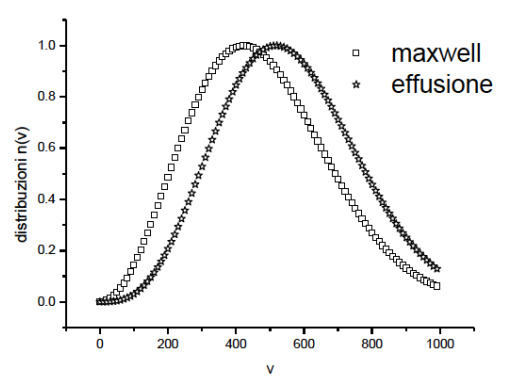
\includegraphics[width=0.5\linewidth]{immagini/effusione}
	\label{fig:effusione}
\end{figure}
		\newline $dn_{effusione} = NF(v)dv \frac{dA\cos\theta vdt}{V} =$ numero di particelle con velocità $v \in (v,v+dv)$ nel cilindretto vicino all'apertura $\Rightarrow dn_e = Nv^2 e^ {-\frac{mv^2}{2K_BT}v\Phi_0}$ \newline
		$dn_e =$ N * la P(di avere $v$) * la P(distanza giusta per uscire) * la P(direzione giusta per uscire)
\begin{figure}[h]
	\centering
	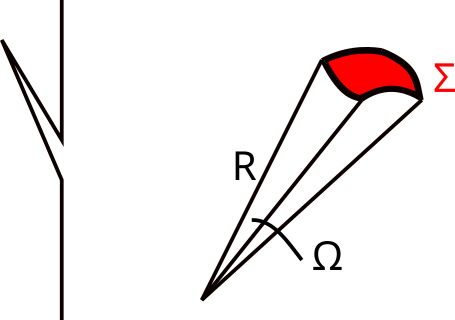
\includegraphics[width=0.3\linewidth]{immagini/angolo solido}
	\caption{Angolo solido}
	\label{fig:angolo-solido}
\end{figure}
		\newline $d\Omega = \frac{dA\cos\theta}{{vdt}^2} \Rightarrow p = \frac{d\Omega}{4\pi} = \frac{dA\cos\theta}{4\pi{vdt}^2}$ \newline
 		$v_{mrs}^e = \sqrt{\frac{4K_BT}{m}} > v_{mrs}$		
		
	\subsection{Effetto Doppler termico}
	
\chapter{Calore specifico solidi}

\section{Teoria Einstein (1906)}
	\begin{enumerate}
	\item Corpo solido è composto da oscillatori indipendenti
	\item Le 3 dimensioni sono indipendenti
	\item Tutti gli oscillatori hanno stessa frequenza $\nu = \frac{1}{2\pi} \sqrt{\frac{b}{m}}$
	\end{enumerate}
	
	\begin{displaymath}
		U = N * \overline{E} * 3 \qquad \overline{E} = \frac{h\nu}{e^{\frac{h\nu}{KT}}-1}
	\end{displaymath}
	$N = n\textsubscript{moli} N_A$ \qquad $R = N_AK_B$ \newline
	\begin{displaymath}
		C_v = \frac{1}{n\textsubscript{moli}} (\frac{\delta U}{\delta T})_{v=cost} = 3N_A \frac{(-e^{\frac{h\nu}{KT}})(-\frac{h\nu}{KT^2})}{(e^{\frac{h\nu}{KT}}-1)^2}h\nu \textcolor{red}{\frac{K_B}{K_B}} = 3R {\frac{h\nu}{KT}}^2\frac{e^{\frac{h\nu}{KT}}}{{(e^{\frac{h\nu}{KT}}-1)}^2}
	\end{displaymath}
	Temperatura di Einstein: \qquad $\theta_E = \frac{h\nu}{K}$
	\begin{equation}
		C_v = 3R {\frac{\theta_E}{T}}^2\frac{e^{\frac{\theta_E}{T}}}{{(e^{\frac{\theta_E}{T}}-1)}^2}
	\end{equation}
	Se $T >> \theta_E \Rightarrow \frac{\theta_E}{T} \to 0 \qquad C_v = 3R$  \newline
	Se $T << \theta_E \Rightarrow C_v \to 0 \qquad \sim e^{-\frac{\theta_E}{T}}$

\section{Modello di Debye}
	\begin{enumerate}
		\item Vibrazioni terminche $\sim$ onde sonore
		\item Solido $\Rightarrow$ continuo elastico
		\item Esistono modi di vibrazione
	\end{enumerate}

	\begin{displaymath}
		\begin{split}
		&g(\nu)d\nu = \frac{4 \pi V}{v^3}\nu^2 d\nu \qquad \mbox{$v$ velocità di propagazione del suono nel mezzo} \\
	    &g(\nu)d\nu= \frac{4 \pi V}{v\textsubscript{long}}\nu^2 d\nu + \frac{4 \pi V}{v\textsubscript{trasv}}\nu^2 d\nu 2
	    \end{split}
	\end{displaymath}

	\begin{equation}
		G(\nu)d\nu = 4\pi V\nu^2 [\underbrace{\frac{1}{v^2_L}+\frac{2}{v^3_t}}_{\frac{1}{\overline{v^3_s}}}]
	\end{equation}
	
	$\int_{0}^{\nu_D} G(\nu)d\nu = 3N$ \qquad 3N: numero massimo di modi
	
		\begin{gather}
		\frac{4\pi V}{{\overline{v_s}}^3} = \frac{9N}{\nu^3_D} \\
		\nu^3_D = \frac{9N\overline{v_s}^3}{4\pi V} \nonumber
		\end{gather}
\begin{figure}[h]
	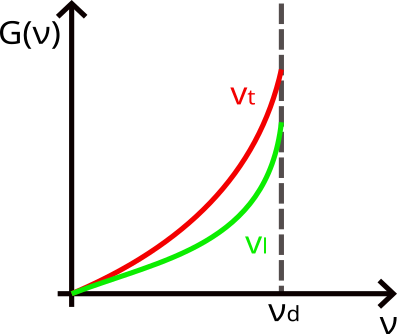
\includegraphics[width=0.3\linewidth]{immagini/1}
	\label{fig:1}
\end{figure}

\end{document}